\documentclass[a4paper,14pt]{extarticle}

\usepackage{cmap}
\usepackage[T2A]{fontenc}
\usepackage[utf8x]{inputenc}
\usepackage[english, russian]{babel}

\usepackage{misccorr} % в заголовках появляется точка, но при ссылке на них ее нет
\usepackage{amssymb,amsfonts,amsmath,amsthm}  
\usepackage{indentfirst}
\usepackage[usenames,dvipsnames]{color} 
\usepackage[unicode,hidelinks]{hyperref}
% \hypersetup{%
%     pdfborder = {0 0 0}
% }

\usepackage{makecell,multirow} 
\usepackage{ulem}
\usepackage{graphicx,wrapfig}
\graphicspath{{img/}}
\usepackage{geometry}
\geometry{left=2cm,right=2cm,top=3cm,bottom=3cm,bindingoffset=0cm,headheight=15pt}
\usepackage{fancyhdr} 
\linespread{1.05} 
\frenchspacing 
\renewcommand{\labelenumii}{\theenumii)} 
\newcommand{\mean}[1]{\langle#1\rangle}
% \usepackage{caption}
%%%%%%%%%%%%%%%%%%%%%%%%%%%%%%%%%%%%%%%%%%%%%%%%%%%%%%%%%%%%%%%%%%%%%%%%%%%%%%%
%%%%%%%%%%%%%%%%%%%%%%%%%%%%%%%%%%%%%%%%%%%%%%%%%%%%%%%%%%%%%%%%%%%%%%%%%%%%%%%

\def\labauthors{Есюнин Д.В., Есюнин М.В.}
\def\labgroup{440}
% \def\department{Кафедра электроники и квантовой физики}
\def\labnumber{1}
\def\labtheme{Исследование твердотельных структур \\[0.2em] методом ЭПР-спектроскопии}

%%%%%%%%%%%%%%%%%%%%%%%%%%%%%%%%%%%%%%%%%%%%%%%%%%%%%%%%%%%%%%%%%%%%%%%%%%%%%%%
%применим колонтитул к стилю страницы
\pagestyle{fancy} 
%очистим "шапку" страницы
\fancyhead{} 
%слева сверху на четных и справа на нечетных
\fancyhead[L]{\labauthors} 
%справа сверху на четных и слева на нечетных
%\fancyhead[R]{Отчёт по лабораторной работе №\labnumber} 
%очистим "подвал" страницы
\fancyfoot{} 
% номер страницы в нижнем колинтуле в центре
\fancyfoot[C]{\thepage} 
\renewcommand{\phi}{\varphi}
%%%%%%%%%%%%%%%%%%%%%%%%%%%%%%%%%%%%%%%%%%%%%%%%%%%%%%%%%%%%%%%%%%%%%%%%%%%%%%%

\usepackage{float}
\usepackage[mode=buildnew]{standalone}
\usepackage{tikz} 
% \usepackage{subcaption}
\usepackage{tikz,csvsimple}
\usetikzlibrary{scopes}
\usetikzlibrary{%
	decorations.pathreplacing,%
	decorations.pathmorphing,%
	patterns,%
	calc,%
	scopes,%
	arrows,%
	% arrows.spaced,%
}
\makeatletter
\newif\if@gather@prefix 
\preto\place@tag@gather{% 
	\if@gather@prefix\iftagsleft@ 
	\kern-\gdisplaywidth@ 
	\rlap{\gather@prefix}% 
	\kern\gdisplaywidth@ 
	\fi\fi 
} 
\appto\place@tag@gather{% 
	\if@gather@prefix\iftagsleft@\else 
	\kern-\displaywidth 
	\rlap{\gather@prefix}% 
	\kern\displaywidth 
	\fi\fi 
	\global\@gather@prefixfalse 
} 
\preto\place@tag{% 
	\if@gather@prefix\iftagsleft@ 
	\kern-\gdisplaywidth@ 
	\rlap{\gather@prefix}% 
	\kern\displaywidth@ 
	\fi\fi 
} 
\appto\place@tag{% 
	\if@gather@prefix\iftagsleft@\else 
	\kern-\displaywidth 
	\rlap{\gather@prefix}% 
	\kern\displaywidth 
	\fi\fi 
	\global\@gather@prefixfalse 
} 
\newcommand*{\beforetext}[1]{% 
	\ifmeasuring@\else
	\gdef\gather@prefix{#1}% 
	\global\@gather@prefixtrue 
	\fi
} 
\makeatother

\usepackage{booktabs}
\usepackage{pgfplots, pgfplotstable}

\usepackage[outline]{contour}
\usepackage{tocloft}
\renewcommand{\cftsecleader}{\cftdotfill{\cftdotsep}} % for parts
% \renewcommand{\cftchapleader}{\cftdotfill{\cftdotsep}} % for chapters
\usepackage{pgfplots,pgfplotstable,booktabs,colortbl}
\pgfplotsset{compat=newest}
\usepackage{physics}
\usepackage{mathtools}
\mathtoolsset{showonlyrefs=true}
\newcommand\Smat{\hat { \mathbf { S } }}

\newcommand*\dotvec[1][1,1]{\crossproducttemp#1\relax}
\def\crossproducttemp#1,#2\relax{{\qty[\vec{#1}\times\vec{#2}\,]}}

\newcommand*\prodvec[1][1,1]{\crossproducttempa#1\relax}
\def\crossproducttempa#1,#2\relax{{\qty[{#1}\times{#2}\,]}}

% \def\E{\mathscr{E}_H}
\def\Rdim{\,\frac{\text{м}^3}{\text{А} \cdot \text{с}}}

\renewcommand{\vec}{\mathbf} % for parts

\begin{document}

\begin{titlepage}
	
	\begin{center}
		
		
		\textsc{Нижегородский государственный университет имени Н.\,И. Лобачевского}
		\vskip 4pt \hrule \vskip 8pt
		\textsc{Радиофизический факультет}
		
		\vfill
		
		{\Large\labtheme}
		
	\end{center}
	
	\vfill
	
	\begin{flushright}
		{Работу выполнили студенты\\ \labauthors\\ 440 группы}
	\end{flushright}
	
	\vfill
	
	\begin{center}
		Нижний Новгород, \the\year
	\end{center}
\end{titlepage}
%\tableofcontents
\newpage


% \section{Теоретическая часть}

\addcontentsline{toc}{section}{Введение}
\section*{Введение}
В настоящей работе исследуется электронный парамагнитный резонанс (ЭПР) -- явление резонансного поглощения энергии электромагнитного поля системой парамагнитных частиц\footnote{Парамагнитные частицы представляют собой вещества, у которых магнитные свойства обуславливаются нескомпенсированным спиновым моментом.}, помещенных в постоянное магнитное поле и взаимодействующих с переменным высокочастотным полем.

В работе исследовалось два образца: \textit{дифенил} и \textit{кристалл рубидия} с активными ионами хрома, у которых нескомпенсированность спинового момента обусловлена неспаренными электронами внешней оболочки. 

Как показано в \cite[стр. 20, 24]{mar}, на данной лабораторной установке может наблюдаться один резонансный переход для дифенила и два -- для кристалла рубидия.


\paragraph{Установка.} СВЧ-излучение, созданное генератором клистронного типа, через волноводный тракт, развязанный с генератором вентилем, подается на волноводный двойной тройник, присоединенный к балансному плечу с аттенюатором, детектору для регистрации мощности сигнала в тракте и непосредственно в резонатор с исследуемым образцом. При этом длина излучаемой волны $\lambda \sim 3$ см.

Резонатор размещен так, что возбужденное в нем СВЧ-поле $\vec{H}_1$ перпендикулярно полю электромагнита $\vec{H}_0$. В результате взаимодействия поля с парамагнетиком возникает сигнал, который измеряется посредством детектора.

За счет наличия балансного плеча, изменяя амплитуду и фазу отражённого в этом плече сигнала, можно наблюдать на продетектированном сигнале как кривую поглощения, так и кривую дисперсии, в зависимости от соотношения фаз сигналов: отраженного от плеча и из резонатора \cite[стр. 33]{mar}.

\paragraph{Общий метод измерений.} Перед началом измерений проводится настройка волноводного тракта: подбирается частота клистронного генератора для максимума мощности в зоне (при $\alpha=0$)\footnote{$\alpha$ -- коэффициент введения аттенюатора}, подвижной стенкой юстируется резонатор по минимуму сигнала (при $\alpha=1$). 

Далее весь анализ, как качественный, так и количественный, ведется на сопоставлении параметров установки и наблюдаемого на осциллографе сигнала с детектора.

\newpage

\newpage
\section{Исследование ЭПР в молекулах дифенила}

Перед началом измерений была проведена настройка тракта, как это описано в выше в введении. После настройки частота СВЧ-колебаний в тракте составила
\begin{equation}
  f_1=9.13 \text{ ГГц}
\end{equation}
Далее был включён электромагнит, задающий постоянное магнитное поле. Измерение тока через катушки электромагнита при наблюдении резонансного перехода на осциллограмме позволяет найти по градуировочной характеристике электромагнита резонансное значение поля:
\begin{equation}
  I_\text{рез}=0.167\pm 0.01 \text{ А}  \quad\Rightarrow\quad
  H_\text{рез}=3700\pm 22\text{ Гс}
\end{equation}

\subsection{Кривые поглощения и дисперсии сигнала ЭПР}
При выключенном волноводном аттенюаторе перенастройка балансного плеча дала возможность наблюдать кривую поглощения $\chi''$ и кривую дисперсии $\chi'$:

\begin{figure}[h!]
    \centering
    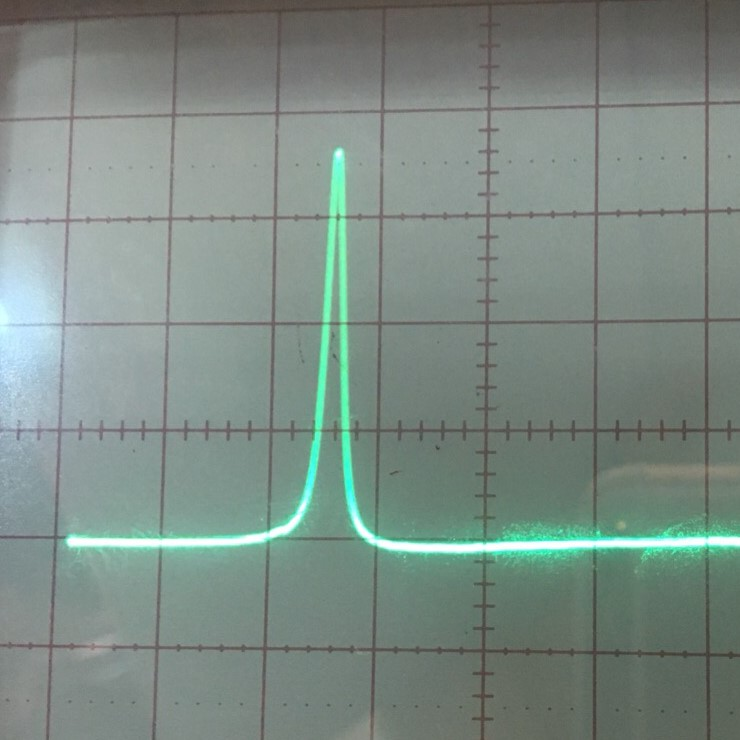
\includegraphics[width=0.49\linewidth]{photo/absorption_curve.jpg}
    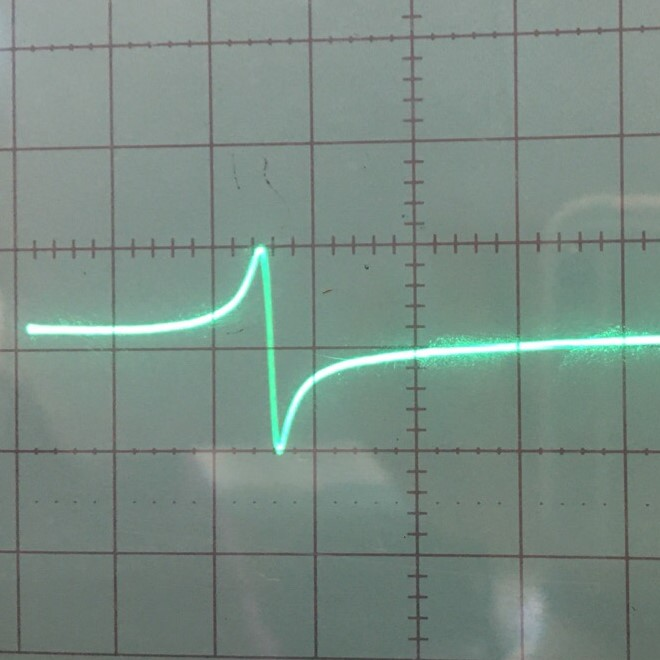
\includegraphics[width=0.49\linewidth]{photo/dispersion_curve.jpg}
    \caption{Кривая $\chi'$, кривая $\chi''$}
    \label{fig:2}
\end{figure}

\subsection{Измерение ширины линии поглощения сигнала ЭПР}

Для измерения ширины в единицах поля было необходимо проградуировать шкалу развертки осциллографа в единицах магнитного поля. Сигнал смещается по горизонтальной оси на величину, пропорциональную изменению постоянного магнитного поля. 

Определяя соответствующие изменения поля $H_0$ по известной зависимости поля от тока $H_0(I)$, можно найти численный коэффициент связи (коэффициент пропорциональности) между изменением поля $\Delta H_0$ и относительном смещением любой точки сигнала по горизонтальной шкале осциллографа $\Delta L$.

При смещении сигнала на $\Delta L=30 \text{ делений}$ изменение тока составило $\Delta I=0,009 \text{ А}$, что соответствует изменению поля $\Delta H_0=200 \text{ Гс}$. Ширина линии поглощения в единицах развертки составляет $\delta L=2 \text{ деления}$, а в единицах поля 

\begin{equation}
  \delta H = \frac{\Delta H\cdot \delta L}{\Delta L}=\frac{200 Гс\cdot 2}{30}\approx 13 \text{ Гс}
\end{equation}

\subsection{Расчет ширины линии в единицах частоты}
Считая, что теоретическая однородная ширина линии в дифениле составляет $2.7$ эрстеда, можно найти время поперечной релаксации $T_2$ :
\begin{equation}
  \delta \omega \approx \frac{2}{T_2} \quad \Rightarrow \quad
  T_2 \approx \frac{2}{\delta \omega} 
\end{equation}
Связь $\delta \omega$ и $\delta H$ можно найти из условия ЭПР при спине $\frac12$:
\begin{equation}
  \hbar \omega = g \beta_B H,
\end{equation}
где $g$-фактор для дифенила можно принять равным двум \cite[стр. 16]{mar}, тогда экспериментальное значение ширины линии и время поперечной релаксации
\begin{equation}
  \delta \omega = \frac{g\beta_B}{\hbar} \delta H = \frac{|e|}{m_e c} \delta H = 2.34 \cdot 10^8 \,\,\frac{\text{рад}}{\text{с}}
  \quad \Rightarrow \quad
  T_2 \approx 8.6 \text{ нс}
\end{equation}
и теоретические 
\begin{equation}
  \delta \omega = \frac{g\beta_B}{\hbar} \delta H = \frac{|e|}{m_e c} \delta H = 0.47 \cdot 10^8 \,\,\frac{\text{рад}}{\text{с}}
  \quad \Rightarrow \quad
  T_2 \approx 40 \text{ нс}
\end{equation}

Из сравнения полученных данных и рассчитанных теоретически, можно заключить, что в эксперименте присутствовало неоднородное уширение линии. 

\subsection{Определение числа парамагнитных частиц в образце, помещенном в резонатор}

При такой настройке балансного плеча, что наблюдается кривая поглощения $\chi''$, детектированный ток имеет вид \cite[стр. 33]{mar}
\begin{equation}
    \label{eq:15}
    i_{\text{дет}} \simeq S P_n \cdot 4 \pi Q \eta \chi''.
\end{equation}

Введем технический коэффициент $A$, характеризующий коэффициент усиления тракта <<детектор-усилитель-осциллограф>>. Его величину можно измерить, подавая известный по величине модулированный СВЧ-сигнал на детекторную головку и измеряя при этом амплитуду видеосигнала на экране осциллографа. Для калибровки тракта усиления использовали режим модуляции СВЧ-генератора меандром. Такой режим модуляции позволяет получить в схеме возбуждение резонатора переменным СВЧ-сигналом, амплитудный размах которого будет совпадать с реализованным ранее случаем непрерывного возбуждения. Таким образом, регистрация СВЧ-меандра как искусственно вводимого в систему эталонного переменного сигнала позволяет по существу прокалибровать вертикальную ось шкалы осциллографа и позволяет провести сравнение эталонного размаха меандром $L_M$ и наблюдаемого сигнала поглощения $L_C$. Коэффициент усиления $A$ будет равен  $\frac{L_M}{P_M}$. Если учесть такого рода амплитудную калибровку, высота сигнала ЭПР на экране осциллографа может быть записана как
\begin{equation}
    \label{eq:16}
    L_{C} = A P_n \cdot 4 \pi Q \eta \chi''(\omega_{0})
\end{equation}

Коэффициент заполнения $\eta$ определяется как отношение  двух интегралов вида  $\int H_{1}^2 \dd{\nu}$ по объему образца и резонатора соответственно. В условиях данной ЭПР-установки
с достаточной степенью точности можно считать 
\begin{equation}
    \label{eq:17}
    \eta \simeq \frac{2 V_{\text{обр}}}{V_{\text{рез}}}.
\end{equation}

Значение $\chi''$ для малых полей  $H_{1}$ при $\omega = \omega_{0}$ можно записать в виде
\begin{equation}
    \label{eq:18}
    \chi '' (\omega_{0}) = \frac{N_{0} \mu^2}{3KT} \omega_{0} T_2^*
\end{equation}

Отсюда количество парамагнитных частиц [на единицу объема] можно оценить как
\begin{equation}
    \label{eq:20}
    N_0 = 3KT \frac{\chi''(\omega_{0})}{\mu^2 \omega_0 T_2^*}.
\end{equation}

Сопоставляя \eqref{eq:16} и \eqref{eq:20}, получаем
\begin{equation}
    \label{eq:21}
    N_0 = \frac{3KT}{8\pi Q \mu^2 \omega_{0} T_2^*} \cdot \frac{L_C}{L_M}  \cdot \frac{P_M}{P_n} \cdot \frac{V_{\text{рез}}}{V_{\text{обр}}}
\end{equation}

Для рассматриваемой установки $Q=5000$, $\frac{V_\text{рез}}{V_\text{обр}} \approx 200$ для образца дифенила, $ \frac{P_M}{P_n}\approx1$, $\mu - \text{ магнетон Бора}$.

Измерив значение модулированного сигнала $L_M=0.52$ В и значение сигнала ЭПР $L_c=0.02$ В, можем рассчитать значение $N_0$:

\begin{equation}
  N_0 = \frac{3\cdot [1.38\cdot10^{-16} \text{ эрг}\cdot\text{K}^{-1}]\cdot [300 \text{ K}]\cdot 200}{8\pi \cdot 5000 \cdot [8.6\cdot 10^{-41} \text{ эрг}^2\text{ Гс}^{-2}]\cdot [2\pi\cdot 9.13\cdot 10^9 \text{ Гц} ]\cdot [6.5 \cdot 10^{-9} \text{ с}]}\cdot \frac{4.4\cdot 0.005 \text{ В}}{4.4\cdot 0.2 \text{ В}}
\end{equation}

Расчетное значение составило $N_0=1.16\cdot 10^{20} \text{ Гс}^2 \text{ эрг}^{-1}=1.16\cdot 10^{20} \text{ см}^{-3}$.


\section{Исследование ЭПР в кристалле рубина}

Аналогично эксперименту с образцом дифенила была проведена настройка тракта. После настройки частота СВЧ-колебаний в тракте составила
\begin{equation}
  f_2=9.13 \text{ ГГц}
\end{equation}
Измерив ток через катушки электромагнита при наблюдении двух резонансных переходов на осциллограмме, по градуировочной характеристике электромагнита были найдены резонансные значения поля:
\begin{equation}
  I_\text{рез1}=0.037 \text{ А}  \quad\Rightarrow\quad
  H_\text{рез1}=850 \text{ Гс}
\end{equation}
\begin{equation}
  I_\text{рез2}=0.160 \text{ А}  \quad\Rightarrow\quad
  H_\text{рез2}=3600 \text{ Гс}
\end{equation}

% \subsection{Получение сигналов ЭПР для случая, когда ось кристалла ориентирована параллельно направлению постоянного магнитного поля}
%  Для получения на экране осциллографа сигналов ЭПР были произведены те же действия, что и для первого эксперимента с дифенилом.

%  Идентификация сигналов ЭПР, наблюдаемых в кристалле рубина:

Так как в кристалле рубина есть два возможных перехода и, соответственно, два резонансных значения поля, идентифицировать сигналы можно по значению поля. 

Для перехода $3/2 \rightarrow 1/2$ резонансное поле имеет вид \cite[стр. 24]{mar}
\begin{equation}
  H_0^{(1)} = \frac{2|D| - \hbar\omega}{g\beta_B} = 
              \frac{2\pi\hbar(2|D|/(2\pi\hbar) - f_2)}{g\beta_B}=
              \frac{2\pi\hbar}{g\beta_B}\cdot 2.3 \text{ ГГц}\approx 820 \text{ Гс}
\end{equation}
где $D/(2\pi \hbar)=5.736\text{ ГГц}$.
А для перехода $-1/2 \rightarrow 1/2$ \cite[стр. 24]{mar}
\begin{equation}
  H_0^{(2)} = \frac{\hbar\omega}{g\beta_B} = \frac{2\pi\hbar}{g\beta_B}f_2 =
  \frac{2\pi\hbar}{g\beta_B}\cdot 9.13 \text{ ГГц}\approx 3188 \text{ Гс}
\end{equation}
Следовательно, для перехода $-1/2 \rightarrow 1/2$ резонансное поле больше, чем для $3/2 \rightarrow 1/2$.


\subsection{Ширина линии поглощения перехода $3/2 \rightarrow 1/2$}
Ширина была измерена аналогично ширине линии поглощения дифенила. Сдвиг сигнала на $\Delta L=15 \text{ делений}$, соотвествует изменению тока $\Delta I=0,007 \text{ А}\to  \Delta H=155 \text{ Гс}$.

Измеренная ширина $\delta L=4.5 \text{ деления}$, тогда
\begin{equation}
\delta H = \frac{\Delta H\cdot \delta L}{\Delta L}=\frac{155 Гс\cdot 4.5}{15}\approx 47 \text{ Гс}
\end{equation}

Тогда можно найти ширину в единицах частоты и выразить время поперечной релаксации:
 \begin{equation}
  \delta \omega = \frac{g\beta_B}{\hbar} \delta H = \frac{|e|}{m_e c} \delta H = 0.82 \cdot 10^9 \,\,\frac{\text{рад}}{\text{с}}
  \quad \Rightarrow \quad
  T_2 = \frac{2}{\delta \omega} \approx 2.34 \text{ нс}
\end{equation}

\subsection{Измерение отношения интенсивностей сигналов ЭПР}

Измерение интенсивностей переходов по высоте сигнала на экране осциллографа дало:
\begin{equation}
  I_{\frac{-1}{2}\to\frac12} = 6 \text{ у.е.}, \quad
  I_{\frac{3}{2}\to\frac12} = 10 \text{ у.е.} 
  \quad \Rightarrow \quad
  \frac{I_{\frac{-1}{2}\to\frac12}}{I_{\frac{3}{2}\to\frac12}}=0.6\approx 1.66^{-1}
\end{equation}

\subsection{Определение числа парамагнитных частиц}
Для рассматриваемой установки  $Q=5000$, $\frac{V_\text{рез}}{V_\text{обр}} \approx 30$ для кристалла рубина, $ \frac{P_M}{P_n}\approx1$. 

Измерив значение модулированного сигнала $L_M=6.2 \cdot 0.2$ В и значение сигнала ЭПР $L_c=2\cdot 0.005$ В, можем рассчитать значение $N_0$:

\begin{equation}
  \frac{3\cdot [1.38\cdot10^{-16} \text{ эрг}\cdot\text{K}^{-1}]\cdot [300 \text{ K}]\cdot 30}{8\pi \cdot 5000 \cdot [8.6\cdot 10^{-41} \text{ эрг}^2\text{ Гс}^{-2}]\cdot [2\pi\cdot 9.162\cdot 10^9 \text{ Гц} ]\cdot [1.5 \cdot 10^{-9} \text{ с}]}\cdot \frac{0.011 \text{ В}}{0.38 \text{ В}}
\end{equation}
Расчетное значение составило $N_0=0.2\cdot 10^{20} \text{ Гс}^2 \text{ эрг}^{-1}=0.2\cdot 10^{20} \text{ см}^{-3}$.

\addcontentsline{toc}{section}{Заключение}
\section*{Заключение}
В настоящей работе мы исследовали спектр поглощения парамагнетиков: дифенила и кристалла рубина (с фиксированной осью кристалла вдоль поля). Для образцов определены вид кривых дисперсии и поглощения, ширины кривых поглощения, частоты резонансного перехода, времена поперечной релаксации и оценено количество парамагнитных частиц.

Сопоставление с теорией позволяет заключить о наличии неоднородного уширения линии поглощения дифенила. Для кристалла рубина теоретические значения резонансного поля по порядку совпадают с экспериментальными.

\begin{thebibliography}{}

  \bibitem{mar} Маругин\,\,А.\,В. Исследование твердотельных структур методом ЭПР-спектроскопии. Н.Новгород: ННГУ, 2008.
\end{thebibliography}

\end{document}